%%%%%%%%%%%%%%%%%%%%%%%%%%%%%%%%%%%%%%%%%%%%%%%%%%%%%%%%%%%%%%%%%%%%%%%%%%%%%
%% INÍCIO CAPÍTULO                                                         %%
%%%%%%%%%%%%%%%%%%%%%%%%%%%%%%%%%%%%%%%%%%%%%%%%%%%%%%%%%%%%%%%%%%%%%%%%%%%%%

\chapter{Análise de algoritmos de ordenação}
\label{cap:2:sorting}

\citacao{%
Nothing in life is to be feared, it is only to be understood. \\ Now is the time to understand more, so that we may fear less.}
{Marie Curie}

\section{Definição formal do problema de ordenação}

O problema de ordenação, como apresentado no Capítulo \ref{cap:1:intro}, é um problema bastante recorrente na Computação.
Sua definição formal consiste em: \\

\textbf{Input: } Uma sequência de n números $(a_1, a_2, a_3,\ldots, a_n)$ \\

\textbf{Output: } Uma reordenação $(a_1, a_2, a_3,\ldots, a_n)$ da sequência para qual \\
$a_1 \leq a_2 \leq a_3 \leq \cdots \leq a_n$. \\

Para este algoritmo, foram pensadas diversas soluções e neste capítulo, será realizado o estudo e compreensão das
mesmas. É importante perceber que, podemos aproximar a ordem de crescimento do algoritmo de ordenação
por inserção de forma bastante precisa utilizando as notações assintóticas, mas não é possível
determinar o tempo de execução para um número de entradas $n$ com muita precisão devido a aspectos
computacionais como:

\begin{itemize}
    \item Chaveamento e prioridade de processo no sistema operacional
    \item Tempo de execução de cada instrução do código compilado
    \item Velocidade de clock inconstante
\end{itemize}

\section{Insertion Sort} \label{cap:2:section:isort}

\subsection{Introdução}

O Insertion Sort é um algoritmo de ordenação relativamente eficiente com número de entradas baixo,
seu funcionamento consiste em consumir o vetor a ser ordenado de forma sequencial buscando pela
localização correta para o elemento no vetor e inserindo-o na mesma.

\subsection{Implementação}

Para o algoritmo de ordenação baseado em inserção, o pseudo-código utilizado para desenvolver o
algoritmo pode ser observado em \ref{insertionSortP}.

\begin{pseudocode}[caption={Algoritmo de ordenação por inserção}, label={insertionSortP}]
INSERTION-SORT(A)
n $\gets$ len(A)
i $\gets$ 2
while i < n do
    j $\gets$ i
    while j > 1 and A[j - 1] > A[j]
        swap(A[j - 1], A[j])
        j $\gets$ j - 1
    i $\gets$ i + 1
\end{pseudocode}

Esse pseudo-código foi implementado na linguagem de programação C 
e pode ser observado no código seguinte:

\begin{lstlisting}[style=CStyle]
void iSort(int * v, int n)
{
    int j, i;
    i = 1;
    while(i < n)
    {
        j = i;
        while(j > 0 && v[j - 1] > v[j])
        {
            swap(&v[j - 1], &v[j]);
            j -= 1;
        }
        i += 1;
    }
}
\end{lstlisting}
    

\subsection{Análise do algoritmo e notação assintótica}

Para que seja determinada a razão de crescimento do algoritmo de ordenação por inserção, é necessário
perceber os tempos de execução de cada linha do pseudo-código \ref{insertionSortP}.
Nesse caso, pode-se ter como base a equação \ref{cap:2:eq:insertionSort:1}.

\begin{equation} \label{cap:2:eq:insertionSort:1}
    T(n) = C_2 + C_3 + \sum_{i=1}^{n}(C_4 + C_5 + C_9) + \sum_{j=1}^{n^2}(C_6 + C_7 + C_8) 
\end{equation}

Portanto, é plausível relacionar \ref{cap:2:eq:insertionSort:1} com \ref{cap:2:eq:insertionSort:2}.

\begin{equation} \label{cap:2:eq:insertionSort:2}
    T(n) = an^2 + bn + c \  para\  a = (C_6 + C_7 + C_8),\  b = (C_4 + C_5 + C_9)\  e\  c = (C_2 + C_3)
\end{equation}

Com isso, pode-se determinar as seguintes notações assintóticas para o algoritmo de ordenação 
por inserção:

\begin{align*} \label{cap:2:eq:insertionSort:3}
    O(n) &= n^x \forall x \geq 2 \\ 
    \Omega(n) &= n^x \forall x \leq 2 \\
    \Theta(n) &= n^2
\end{align*}

\subsection{Comparação teórica-prática}

Para melhor compreensão do tempo de execução do algoritmo de ordenação por inserção, pode-se observar o gráfico
em \ref{cap:2:graph:insertionSort} que apresentam o tempo de execução para o algoritmo de ordenação por inserção
para 2048 casos diferentes com o número de entradas $n$ variando de 1 a 65536.

\begin{figure}[h]
    \centering
    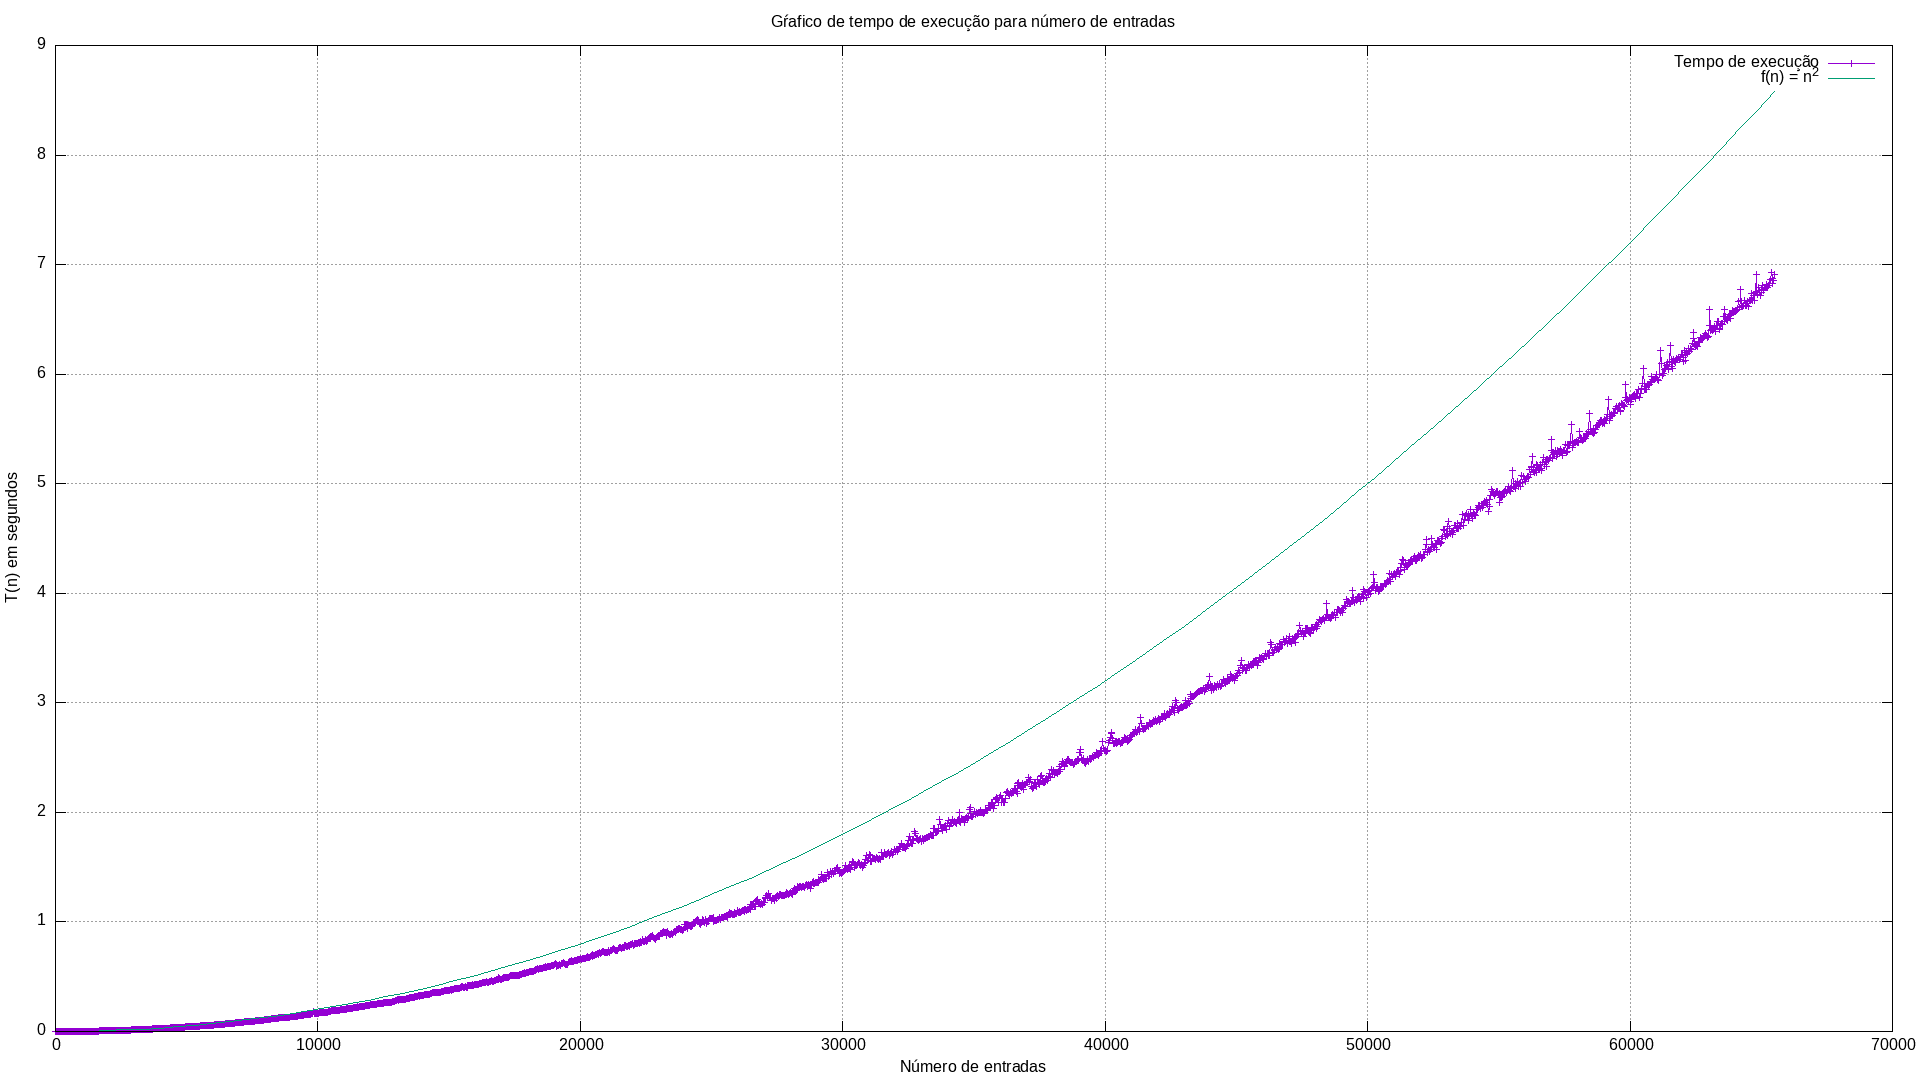
\includegraphics[width=\textwidth]{image/graphics/insertionSort.png}
    \caption{Gráfico com tempo de execução do algoritmo de ordenação por inserção}
    \label{cap:2:graph:insertionSort}
\end{figure}

No gráfico \ref{cap:2:graph:insertionSort}, é possível perceber que o tempo de execução do algoritmo se aproxima
da função $f(n)$ que é uma função quadrática para $n$ com uma redução de escala para melhor percepção e comparação. Então,
utilizando como base o gráfico \ref{cap:2:graph:insertionSort}, pode-se confirmar que a ordem de crescimento determinada é
precisa.

\subsection{Discussão sobre tempo de execução e uso de memória}

Sobre seu tempo de execução, o algoritmo de ordenação por inserção é eficiente para vetores
com poucas entradas a partir de um certo limiar e do contexto, existem outros algoritmos de ordenação
mais eficientes que o mesmo. Sobre seu uso de memória, é constante porque utiliza apenas algumas variáveis
auxiliares.


\section{Selection Sort} \label{cap:2:section:ssort}

\subsection{Introdução}

O Selection Sort é um algoritmo de ordenação relativamente eficiente com número de entradas baixo,
seu funcionamento consiste em consumir o vetor a ser ordenado de forma sequencial buscando pelo menor
elemento do vetor e inserindo-o na posição correta.

\subsection{Implementação}

Para o algoritmo de ordenação baseado em seleção, o pseudo-código utilizado para desenvolver o
algoritmo pode ser observado em \ref{selectionSortP}.

\begin{pseudocode}[caption={Algoritmo de ordenação por seleção}, label={selectionSortP}]
SELECTION-SORT(A)
n $\gets$ len(A)
i $\gets$ 1
while i < n - 1 do
    min $\gets$ i
    j $\gets$ i + 1
    while j < n do
        if A[j] < A[min] then
            min $\gets$ j
    if i $\neq$ min then
        swap(A[i], A[min])
    i $\gets$ i + 1
\end{pseudocode}

Esse pseudo-código foi implementado na linguagem de programação C 
e pode ser observado no código seguinte:

\begin{lstlisting}[style=CStyle]
void sSort(int * v, int n)
{
    int min;
    for (int i = 0; i < n - 1; i++)
    {
        min = i;
        for (int j = i + 1; j < n; j++)
        {
            if (v[j] < v[min])
            {
                min = j;
            }
        }
        if (i != min)
        {
            swap(&v[i], &v[min]);
        }
    }
}
\end{lstlisting}

\subsection{Análise do algoritmo e notação assintótica}

Para que seja determinada a razão de crescimento do algoritmo de ordenação por seleção, é necessário
perceber os tempos de execução de cada linha do pseudo-código \ref{selectionSortP}.
Nesse caso, pode-se ter como base a equação \ref{cap:2:eq:selectionSort:1}.

\begin{equation} \label{cap:2:eq:selectionSort:1}
    T(n) = C_2 + C_3 + \sum_{i=1}^{n - 1}(C_4 + C_5 + C_6 + C_9 + C_{10} + C_{11} + C_{12}) + \sum_{j=1}^{n^2}(C_7 + C_8) 
\end{equation}

Portanto, é plausível relacionar a equação \ref{cap:2:eq:selectionSort:1} com a equação \ref{cap:2:eq:selectionSort:2}.

\begin{equation} \label{cap:2:eq:selectionSort:2}
    T(n) = an^2 + bn + c \  para\  a = (C_7 + C_8),\  b = (C_4 + C_5 + C_6 + C_9 + C_{10} + C_{11} + C_{12})\  e\  c = (C_2 + C_3)
\end{equation}

Com isso, pode-se determinar as seguintes notações assintóticas para o algoritmo de ordenação 
por seleção:

\begin{align*} \label{cap:2:eq:selectionSort:3}
    O(n) &= n^x \forall x \geq 2 \\ 
    \Omega(n) &= n^x \forall x \leq 2 \\
    \Theta(n) &= n^2
\end{align*}

\subsection{Comparação teórica-prática}

Para melhor compreensão do tempo de execução do algoritmo de ordenação por seleção, pode-se observar o gráfico 
\ref{cap:2:graph:selectionSort} que apresentam o tempo de execução para o algoritmo de ordenação por seleção
para 2048 casos diferentes com o número de entradas $n$ variando de 1 a 65536.

\begin{figure}[h]
    \centering
    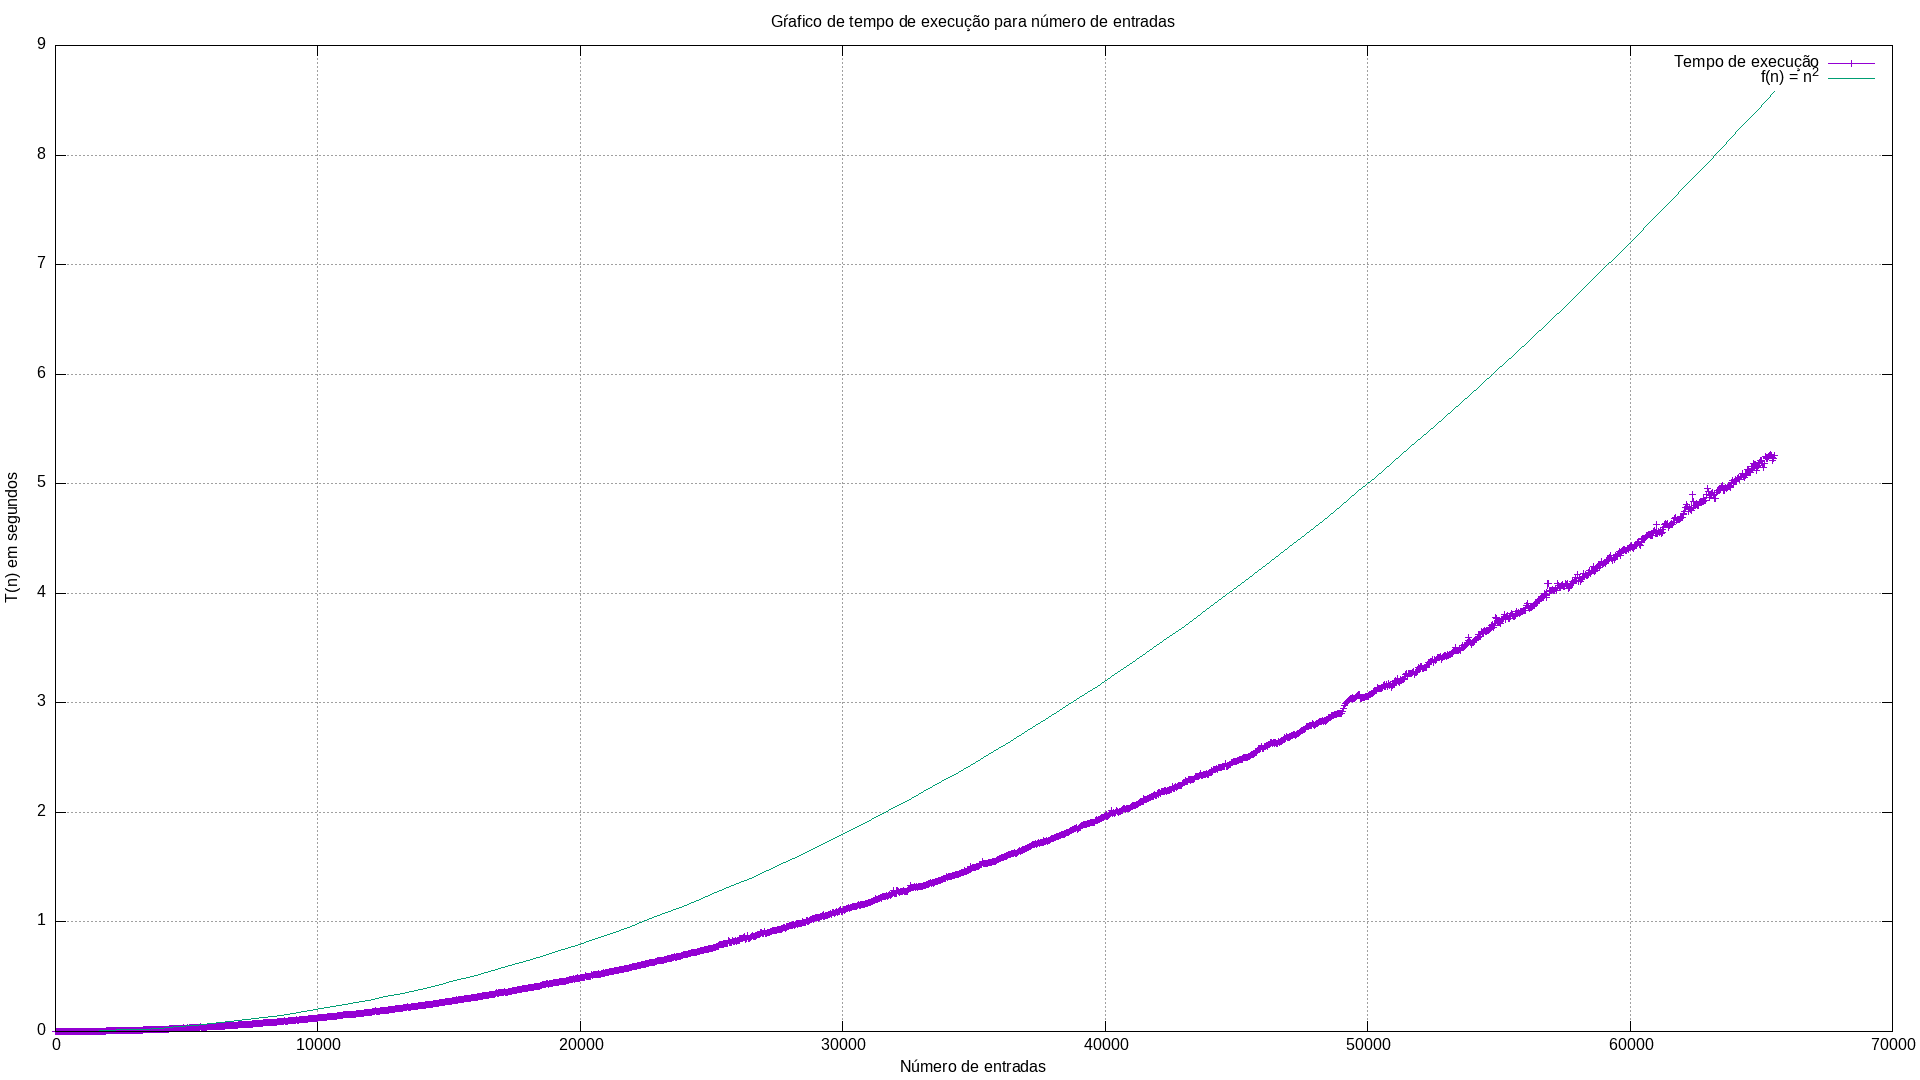
\includegraphics[width=\textwidth]{image/graphics/selectionSort.png}
    \caption{Gráfico com tempo de execução do algoritmo de ordenação por seleção}
    \label{cap:2:graph:selectionSort}
\end{figure}

No gráfico \ref{cap:2:graph:selectionSort}, é possível perceber que o tempo de execução do algoritmo se aproxima
da função $f(n)$ que é uma função quadrática para $n$ com uma redução de escala para melhor percepção e comparação. Então,
utilizando como base o gráfico \ref{cap:2:graph:selectionSort}, pode-se confirmar que a ordem de crescimento determinada é
precisa.

\subsection{Discussão sobre tempo de execução e uso de memória}

Sobre seu tempo de execução, o algoritmo de ordenação por seleção é eficiente para vetores
com poucas entradas a partir de um certo limiar e do contexto, existem outros algoritmos de ordenação
mais eficientes que o mesmo. Sobre seu uso de memória, é constante porque utiliza apenas algumas variáveis
auxiliares.


\section{Heap Sort} \label{cap:2:section:hsort}

\subsection{Introdução}

O \textit{Heap} Sort é um algoritmo de ordenação bastante eficiente, seu funcionamento é baseado
na estrutura de dados chamada \textit{Heap}, que pode ser implementada utilizando um vetor que
mantém as propriedades de \textit{Heap}, seja ela a propriedade de \textit{max-heap} ou a propriedade
de \textit{min-heap}.

\begin{itemize}

    \item \textit{max-heap}: é uma propriedade da estrutura de dados \textit{Heap} que indica que
    a raiz ou primeiro indíce do vetor é o maior elemento da \textit{Heap}.
    \item \textit{min-heap}: é uma propriedade da estrutura de dados \textit{Heap} que indica que
    a raiz ou primeiro indíce do vetor é o menor elemento da \textit{Heap}.

\end{itemize}

\subsection{Implementação}

Para o algoritmo de ordenação baseado na estrutura de uma \textit{Heap}, o pseudo-código utilizado para desenvolver o
algoritmo pode ser observado em \ref{heapSortP}.

\begin{pseudocode}[caption={Algoritmo de ordenação utilizando uma \textit{Heap}}, label={heapSortP}]
HEAP-SORT(A)
n $\gets$ len(A)
BUILD-MAX-HEAP(A)
i $\gets$ n - 1
while i > 1 do
    swap(A[0], A[i])
    MAX-HEAPIFY(A)
    i $\gets$ i - 1
\end{pseudocode}

Esse pseudo-código foi implementado na linguagem de programação C 
e pode ser observado no código seguinte:

\begin{lstlisting}[style=CStyle]
void heapify(int * v, int n, int i)
{

    int largest = i;

    int left = 2 * i + 1;

    int right = 2 * i + 2;

    if (left < n && v[left] > v[largest])
    {
        largest = left;
    }

    if (right < n && v[right] > v[largest])
    {
        largest = right;
    }

    if (largest != i)
    {
        swap(&v[i], &v[largest]);

        heapify(v, n, largest);
    }
}

void hSort(int * v, int n)
{
    int i;

    for (i = n / 2 - 1; i >= 0; i--)
    {
        heapify(v, n, i);
    }

    // Heap sort
    for (int i = n - 1; i > 0; i--) 
    {

        swap(&v[0], &v[i]);

        heapify(v, i, 0);
    }
}
\end{lstlisting}

\subsection{Análise do algoritmo e notação assintótica}

Para que seja determinada a razão de crescimento do algoritmo de ordenação pela estrutura da \textit{Heap}, é necessário
perceber os tempos de execução de cada linha do pseudo-código \ref{heapSortP}.
Nesse caso, pode-se ter como base a equação \ref{cap:2:eq:heapSort:1}.

\begin{equation} \label{cap:2:eq:heapSort:1}
    T(n) = C_2 + T(BUILDMAXHEAP) + C_4 + \sum_{i=2}^{n - 1}(C_6 + T(MAXHEAPIFY) + C_8)
\end{equation}

Sabendo que, o tempo de execução $T(BUILDMAXHEAP) = O(n)$ e o tempo de execução $T(MAXHEAPIFY) = O(\log n)$, podemos assumir
a relação entre a equação \ref{cap:2:eq:heapSort:1} com a equação \ref{cap:2:eq:heapSort:2}.

\begin{equation} \label{cap:2:eq:heapSort:2}
    T(n) = n + an + c\  para\  a = (C_6 + \log n + C_8)\  e\  c = (C_2 + C_4)
\end{equation}

Com isso, pode-se determinar as seguintes notações assintóticas para o algoritmo de ordenação 
pela estrutura da \textit{Heap}:

\begin{align*} \label{cap:2:eq:heapSort:3}
    O(n) &= n \times \log n \\ 
    \Omega(n) &= n \times \log n \\
    \Theta(n) &= n \times \log n
\end{align*}

\subsection{Comparação teórica-prática}

Para melhor compreensão do tempo de execução do algoritmo de ordenação pela estrutura da \textit{Heap}, pode-se observar o gráfico 
\ref{cap:2:graph:heapSort} que apresentam o tempo de execução para o algoritmo de ordenação pela estrutura da \textit{Heap}
para 8192 casos diferentes com o número de entradas $n$ variando de 1 a 1048576.

\begin{figure}[h]
    \centering
    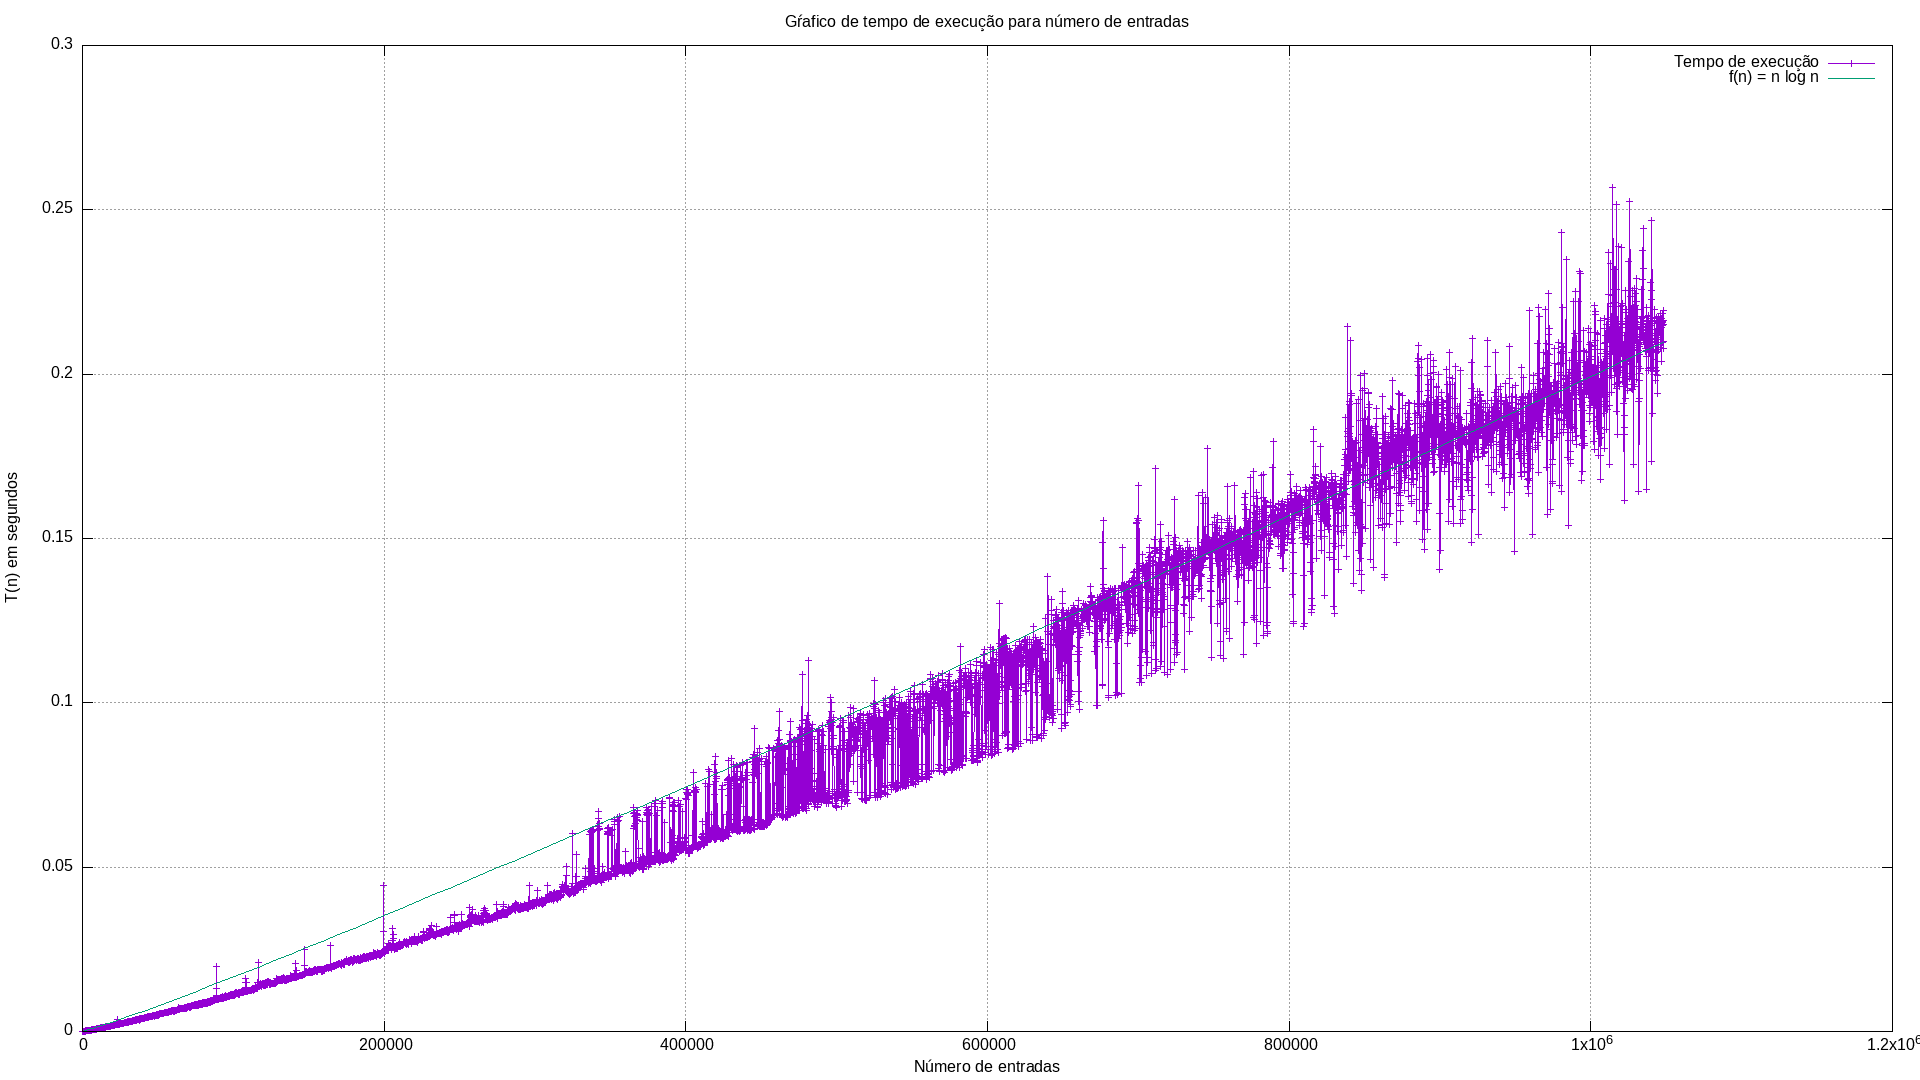
\includegraphics[width=\textwidth]{image/graphics/heapSort.png}
    \caption{Gráfico com tempo de execução do algoritmo de ordenação pela estrutura da \textit{Heap}}
    \label{cap:2:graph:heapSort}
\end{figure}

No gráfico \ref{cap:2:graph:heapSort}, é possível perceber que o tempo de execução do algoritmo se aproxima
da função $f(n)$ que é uma função $n \times \log n$ para $n$ com uma redução de escala para melhor percepção e comparação. Então,
utilizando como base o gráfico \ref{cap:2:graph:heapSort}, pode-se confirmar que a ordem de crescimento determinada é
precisa.

\subsection{Discussão sobre tempo de execução e uso de memória}

Sobre seu tempo de execução, o algoritmo de ordenação pela estrutura da \textit{Heap} é eficiente para
vetores com muitas entradas. Sobre seu uso de memória, é constante porque utiliza apenas algumas variáveis
auxiliares e transfigura o vetor origem de forma direta.


\section{Merge Sort} \label{cap:2:section:msort}

\subsection{Introdução}

O \textit{Merge} Sort é um algoritmo de ordenação bastante eficiente, seu funcionamento é baseado
na estratégia de ordenação de dividir para conquistar. Basicamente, o processo de ordenação consiste
em separar de forma recursiva o vetor, até que contenha 1 elemento e então, realiza o procedimento
\textit{merge}, que consiste produzir um novo vetor ordenado dos elementos de mesma profundidade
topológica.

\subsection{Implementação}

Para o algoritmo de ordenação por mesclagem, o pseudo-código utilizado para desenvolver o
algoritmo pode ser observado em \ref{mergeSortP}.

\begin{pseudocode}[caption={Algoritmo de ordenação por mesclagem}, label={mergeSortP}]
MERGE-SORT(A, l, r)
if l < r then
    m $\gets$ l + (r - l) / 2

    MERGE-SORT(A, l, m)
    MERGE-SORT(A, m + 1, r)

    MERGE(A, l, m, r)
\end{pseudocode}

Esse pseudo-código foi implementado na linguagem de programação C 
e pode ser observado no código seguinte:

\begin{lstlisting}[style=CStyle]
void merge(int * v, int l, int m, int r) 
{ 
    int i, j, k; 
    int n1 = m - l + 1; 
    int n2 = r - m; 

    int L[n1], R[n2]; 
    
    for (i = 0; i < n1; i++) 
        L[i] = v[l + i]; 
    for (j = 0; j < n2; j++) 
        R[j] = v[m + 1 + j]; 
    
    i = 0; 
    
    j = 0; 
    
    k = l; 
    while (i < n1 && j < n2) { 
        if (L[i] <= R[j]) { 
            v[k] = L[i]; 
            i++; 
        } 
        else { 
            v[k] = R[j]; 
            j++; 
        } 
        k++; 
    } 
    
    while (i < n1) { 
        v[k] = L[i]; 
        i++; 
        k++; 
    } 
    
    while (j < n2) { 
        v[k] = R[j]; 
        j++; 
        k++; 
    } 
} 

void mSort(int * v, int l, int r) 
{ 
    if (l < r) { 
        int m = l + (r - l) / 2; 
  
        mSort(v, l, m); 
        mSort(v, m + 1, r); 
  
        merge(v, l, m, r); 
    } 
} 
\end{lstlisting}

\subsection{Análise do algoritmo e notação assintótica}

Para que seja determinada a razão de crescimento do algoritmo de ordenação por mesclagem, é necessário
perceber os tempos de execução de cada linha do pseudo-código \ref{mergeSortP}.
Nesse caso, pode-se ter como base a equação \ref{cap:2:eq:mergeSort:1}.

\begin{equation} \label{cap:2:eq:mergeSort:1}
    T(n) = \sum_{i=1}^{\log n}(C_2 + C_3 + T(MERGE))
\end{equation}

Sabendo que, o tempo de execução $T(MERGE) = O(n)$, podemos assumir a relação entre a equação 
\ref{cap:2:eq:mergeSort:1} com a equação \ref{cap:2:eq:mergeSort:2}.

\begin{equation} \label{cap:2:eq:mergeSort:2}
    T(n) = a \times \log n + c\  para\  a = (C_2 + C_3 + T(MERGE))
\end{equation}

Com isso, pode-se determinar as seguintes notações assintóticas para o algoritmo de ordenação por mesclagem:

\begin{align*} \label{cap:2:eq:mergeSort:3}
    O(n) &= n \times \log n \\ 
    \Omega(n) &= n \times \log n \\
    \Theta(n) &= n \times \log n
\end{align*}

\subsection{Comparação teórica-prática}

Para melhor compreensão do tempo de execução do algoritmo de ordenação por mesclagem, pode-se observar o gráfico 
\ref{cap:2:graph:mergeSort} que apresentam o tempo de execução para o algoritmo de ordenação por mesclagem
para 8192 casos diferentes com o número de entradas $n$ variando de 1 a 1048576.

\begin{figure}[h]
    \centering
    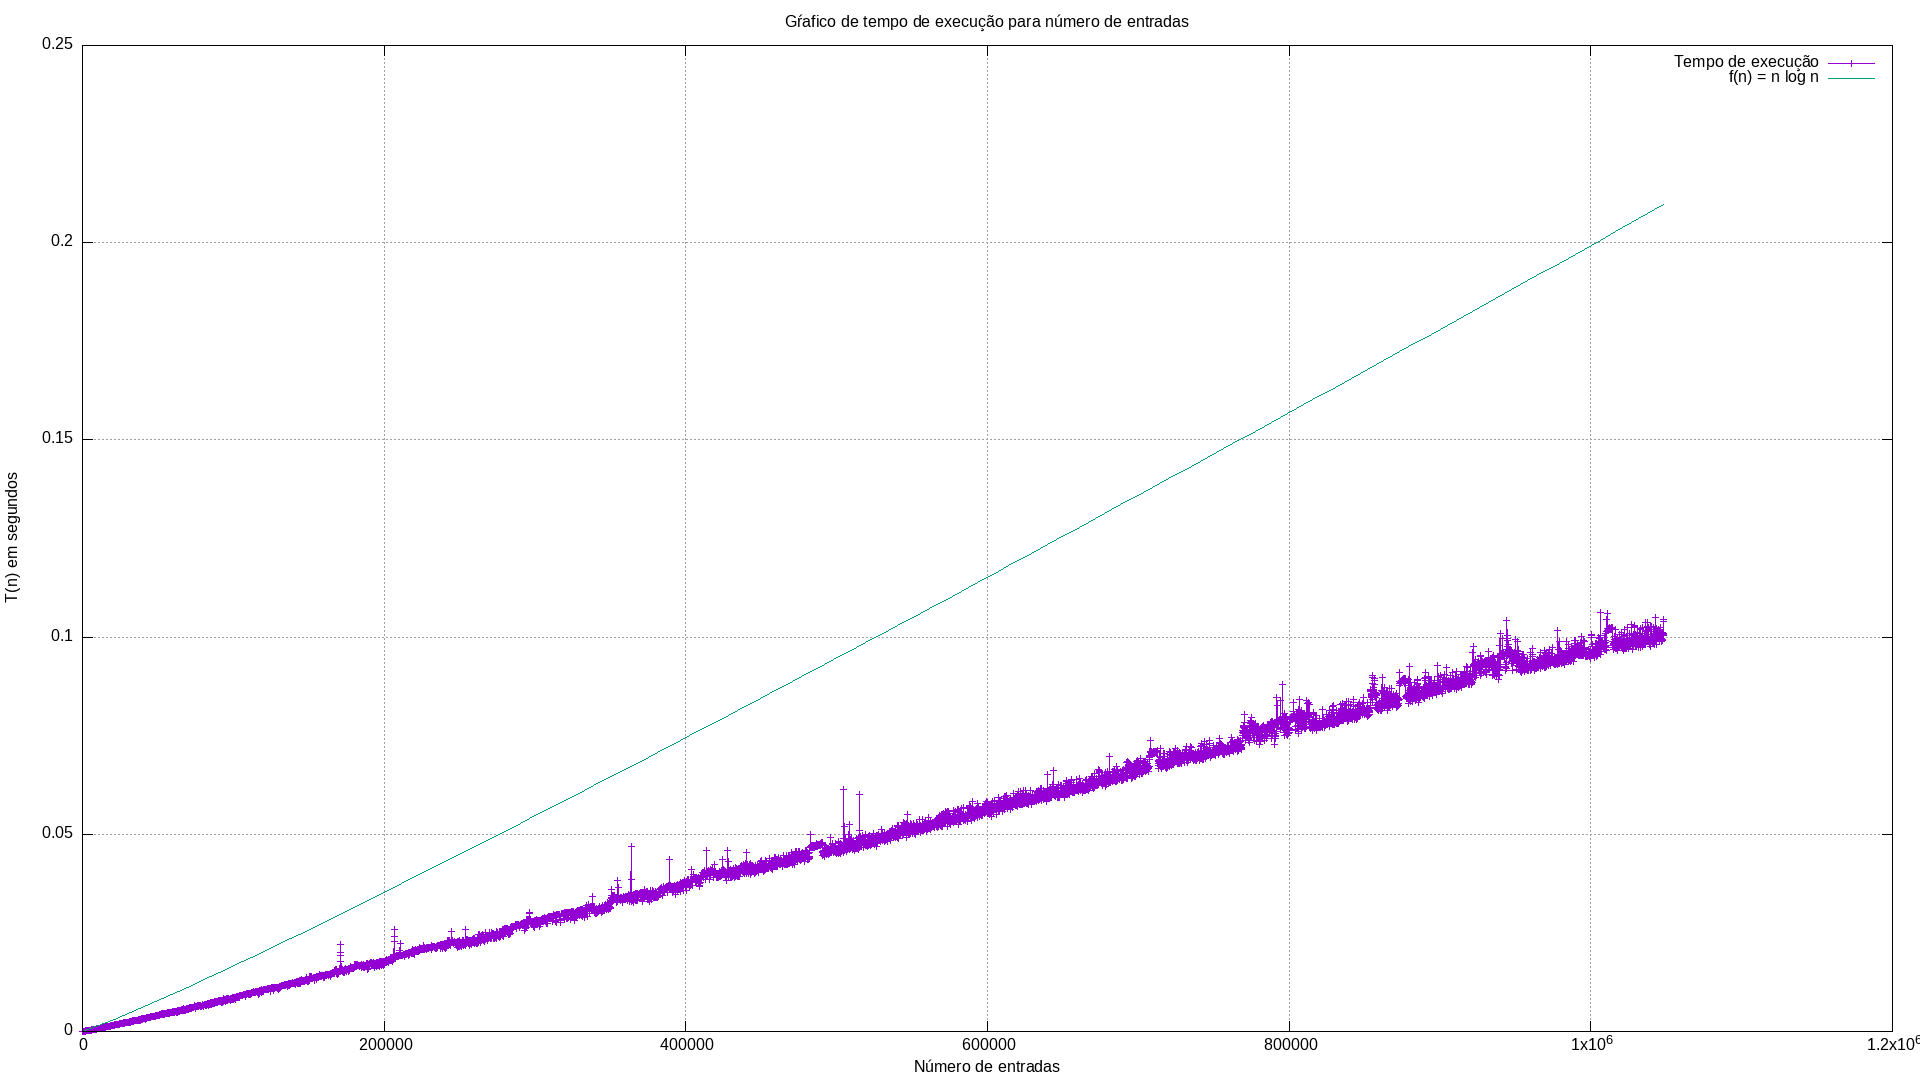
\includegraphics[width=\textwidth]{image/graphics/mergeSort.png}
    \caption{Gráfico com tempo de execução do algoritmo de ordenação por mesclagem}
    \label{cap:2:graph:mergeSort}
\end{figure}

No gráfico \ref{cap:2:graph:mergeSort}, é possível perceber que o tempo de execução do algoritmo se aproxima
da função $f(n)$ que é uma função $n \times \log n$ para $n$ com uma redução de escala para melhor percepção e comparação. Então,
utilizando como base o gráfico \ref{cap:2:graph:mergeSort}, pode-se confirmar que a ordem de crescimento determinada é
precisa.

\subsection{Discussão sobre tempo de execução e uso de memória}

Sobre seu tempo de execução, o algoritmo de ordenação por mesclagem é eficiente para
vetores com muitas entradas. Sobre seu uso de memória, é na ordem de $S(n) = n$ porque utiliza vetores auxiliares
que crescem de forma linear com $n$.


\section{Quick Sort} \label{cap:2:section:qsort}

\subsection{Introdução}

O \textit{Quick} Sort é um algoritmo de ordenação bastante eficiente, seu funcionamento é baseado
na estratégia de ordenação de dividir para conquistar. Basicamente, o processo é particionar um vetor
de forma recursiva enquanto realiza a ordenação nele, utilizando uma lógica de pivot e marcador para
troca.

\subsection{Implementação}

Para o algoritmo de ordenação por particionamento, o pseudo-código utilizado para desenvolver o
algoritmo pode ser observado em \ref{quickSortP} retirado do livro \cite{cormen2022algorithms}.

\begin{pseudocode}[caption={Algoritmo de ordenação por particionamento}, label={quickSortP}]
QUICK-SORT(A, p, r)
if p < r then
    q = PARTITION(A, p, r)
    QUICK-SORT(A, p, q - 1)
    QUICK-SORT(A, q + 1, r)
\end{pseudocode}

Esse pseudo-código foi implementado na linguagem de programação C 
e pode ser observado no código seguinte:

\begin{lstlisting}[style=CStyle]
int partition(int * v, int s, int e)
{

    int pivot = v[s];

    int i = s - 1;
    int j = e + 1;

    while (1)
    {
        do
        {
            i += 1;
        } while (v[i] < pivot);

        do
        {
            j -= 1;
        } while (v[j] > pivot);
        
        if (i >= j)
        {
            return j;
        }

        swap(&v[i], &v[j]);
    }
}

void qSort(int * v, int s, int e)
{
    if (s >= 0 && e >= 0 && s < e)
    {
        int p = partition(v, s, e);
        qSort(v, s, p);
        qSort(v, p + 1, e);
    }
}
\end{lstlisting}

\subsection{Análise do algoritmo e notação assintótica}

Para que seja determinada a razão de crescimento do algoritmo de ordenação por particionamento, é necessário
perceber os tempos de execução de cada linha do pseudo-código \ref{quickSortP}.
Nesse caso, pode-se ter como base a equação \ref{cap:2:eq:quickSort:1}.

\begin{equation} \label{cap:2:eq:quickSort:1}
    T(n) = \sum_{i=1}^{\log n}(C_2 + T(PARTITION))
\end{equation}

Sabendo que, o tempo de execução $T(PARTITION) = O(n)$, podemos assumir a relação entre a equação 
\ref{cap:2:eq:quickSort:1} com a equação \ref{cap:2:eq:quickSort:2}.

\begin{equation} \label{cap:2:eq:quickSort:2}
    T(n) = a \times \log n + c\  para\  a = (C_2 + T(PARTITION))
\end{equation}

Com isso, pode-se determinar as seguintes notações assintóticas para o algoritmo de ordenação por particionamento:

\begin{align*} \label{cap:2:eq:quickSort:3}
    O(n) &= n \times \log n \\ 
    \Omega(n) &= n \times \log n \\
    \Theta(n) &= n \times \log n
\end{align*}

\subsection{Comparação teórica-prática}

Para melhor compreensão do tempo de execução do algoritmo de ordenação por particionamento, pode-se observar o gráfico 
\ref{cap:2:graph:quickSort} que apresentam o tempo de execução para o algoritmo de ordenação por particionamento
para 8192 casos diferentes com o número de entradas $n$ variando de 1 a 1048576.

\begin{figure}[h]
    \centering
    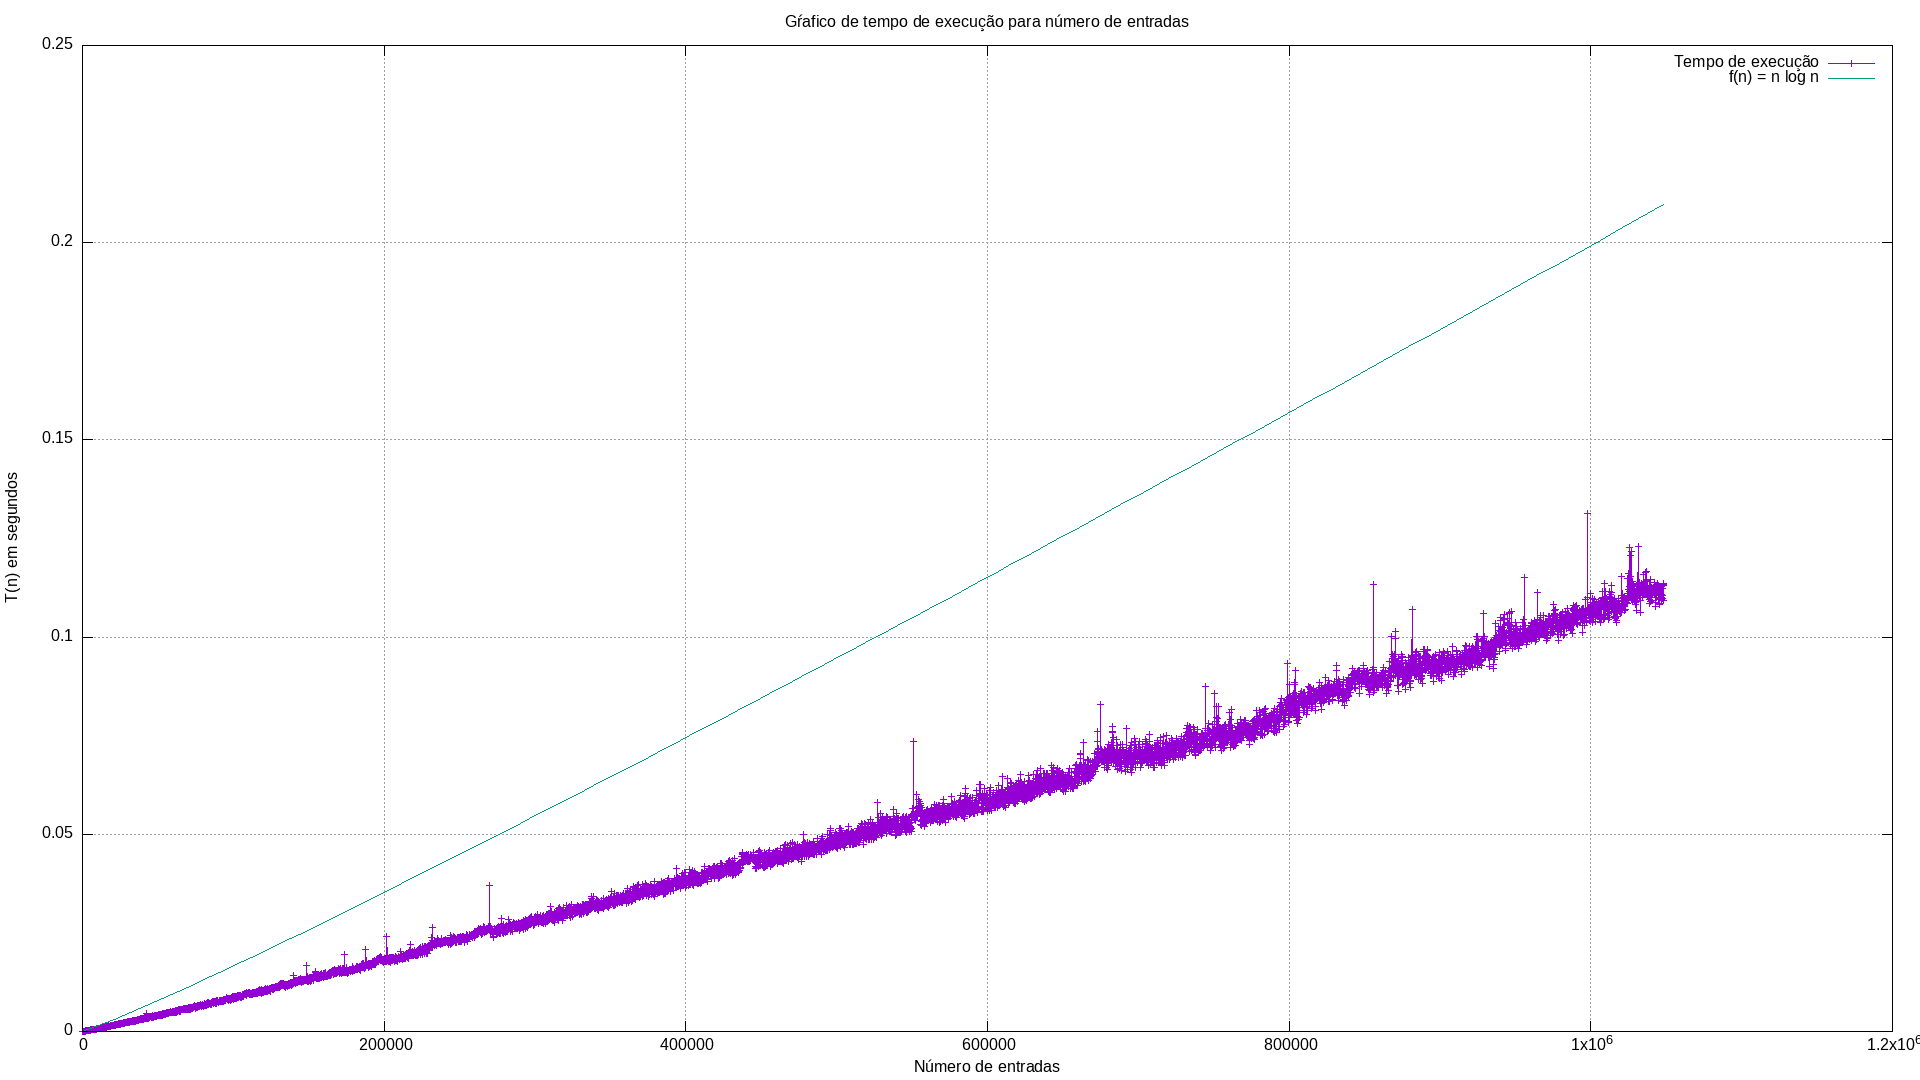
\includegraphics[width=\textwidth]{image/graphics/quickSort.png}
    \caption{Gráfico com tempo de execução do algoritmo de ordenação por particionamento}
    \label{cap:2:graph:quickSort}
\end{figure}

No gráfico \ref{cap:2:graph:quickSort}, é possível perceber que o tempo de execução do algoritmo se aproxima
da função $f(n)$ que é uma função $n \times \log n$ para $n$ com uma redução de escala para melhor percepção e comparação. Então,
utilizando como base o gráfico \ref{cap:2:graph:quickSort}, pode-se confirmar que a ordem de crescimento determinada é
precisa.

\subsection{Discussão sobre tempo de execução e uso de memória}

Sobre seu tempo de execução, o algoritmo de ordenação por particionamento é eficiente para
vetores com muitas entradas. Sobre seu uso de memória, é constante porque utiliza apenas algumas variáveis
auxiliares e transfigura o vetor origem de forma direta.


\section{Counting Sort} \label{cap:2:section:csort}

\subsection{Introdução}

O \textit{Counting} Sort é um algoritmo de ordenação bastante eficiente dada a uma quantidade de
memória equivalente as necessidades. Seu funcionamento é baseado num método de contagem, iterando pelo vetor 
origem e contando as aparições dos elementos num vetor auxiliar $K$.

Uma das características desse algoritmo é, como será apresentado, seu tempo de execução linear mas
sua grande utilização de memória a depender da necessidade. Sendo, seu uso de memória a equação \ref{cap:2:eq:countingSort:0}.

\begin{equation} \label{cap:2:eq:countingSort:0}
    M(n) = n + k \ para \ k = |\min n| + |\max n|
\end{equation}

\subsection{Implementação}

Para o algoritmo de ordenação por contagem, o pseudo-código utilizado para desenvolver o
algoritmo pode ser observado em \ref{countingSortP} retirado do livro \cite{cormen2022algorithms}.

\begin{pseudocode}[caption={Algoritmo de ordenação por contagem}, label={countingSortP}]
COUNTING-SORT(A, n, K)
let B[1:n] and C[0:K] be new arrays
for i $\gets$ 0 to k
    C[i] $\gets$ 0
for j $\gets$ 1 to n
    C[A[j]] $\gets$ C[A[j]] + 1
for i $\gets$ 1 to k
    C[i] = C[i] + C[i - 1]
for j $\gets$ n downto 1
    B[C[A[j]]] $\gets$ A[j]
    C[A[j]] $\gets$ C[A[j]] - 1
return B
\end{pseudocode}

Esse pseudo-código foi implementado na linguagem de programação C 
e pode ser observado no código seguinte:

\begin{lstlisting}[style=CStyle]
void cSort(unsigned char * v, int n)
{
    int i, j;

    int size = __UINT8_MAX__;

    unsigned char B[n];
    int C[size + 1];

    for (i = 0; i < size + 1; i++)
    {
        C[i] = 0;
    }

    for (j = 0; j < n; j++)
    {
        C[v[j]]++;
    }

    for (i = 1; i <= size; i++)
    {
        C[i] = C[i] + C[i - 1];
    }

    for (j = n - 1; j >= 0; j--)
    {
        B[C[v[j]] - 1] = v[j];
        C[v[j]]--;
    }

    for (i = 0; i < n; i++)
    {
        v[i] = B[i];
    }

}
\end{lstlisting}
        

Essa implementação do algoritmo em C, leva em consideração que o vetor
a ser ordenado é de caracteres, portanto, o vetor auxiliar $K$ sempre será
igual a 256, por ser o máximo possível de distância entre o mínimo e o 
máximo do vetor origem.

\subsection{Análise do algoritmo e notação assintótica}

Para que seja determinada a razão de crescimento do algoritmo de ordenação por contagem, é necessário
perceber os tempos de execução de cada linha do pseudo-código \ref{countingSortP}.
Nesse caso, pode-se ter como base a equação \ref{cap:2:eq:countingSort:1}.

\begin{equation} \label{cap:2:eq:countingSort:1}
    T(n) = C_2 + C_{14} + \sum_{i=1}^{n}(C_5 + C_{12} + C_{13}) + \sum_{i=1}^{k}(C_3 + C_8)
\end{equation}

Podemos assumir a relação entre a equação 
\ref{cap:2:eq:countingSort:1} com a equação \ref{cap:2:eq:countingSort:2}.

\begin{equation} \label{cap:2:eq:countingSort:2}
    T(n) = an + bk + c\  para\  a = (C_5 + C_{12} + C_{13}) \ ,b = (C_3 + C_8) \ e \ c = (C_1 + C_{14})
\end{equation}

Com isso, pode-se determinar as seguintes notações assintóticas para o algoritmo de ordenação por contagem:

\begin{align*} \label{cap:2:eq:countingSort:3}
    O(n) &= n + k \\ 
    \Omega(n) &= n + k \\
    \Theta(n) &= n + k
\end{align*}

\subsection{Comparação teórica-prática}

Para melhor compreensão do tempo de execução do algoritmo de ordenação por contagem, pode-se observar o gráfico 
\ref{cap:2:graph:countingSort} que apresentam o tempo de execução para o algoritmo de ordenação por contagem
para 8192 casos diferentes com o número de entradas $n$ variando de 1 a 1048576.

\begin{figure}[h]
    \centering
    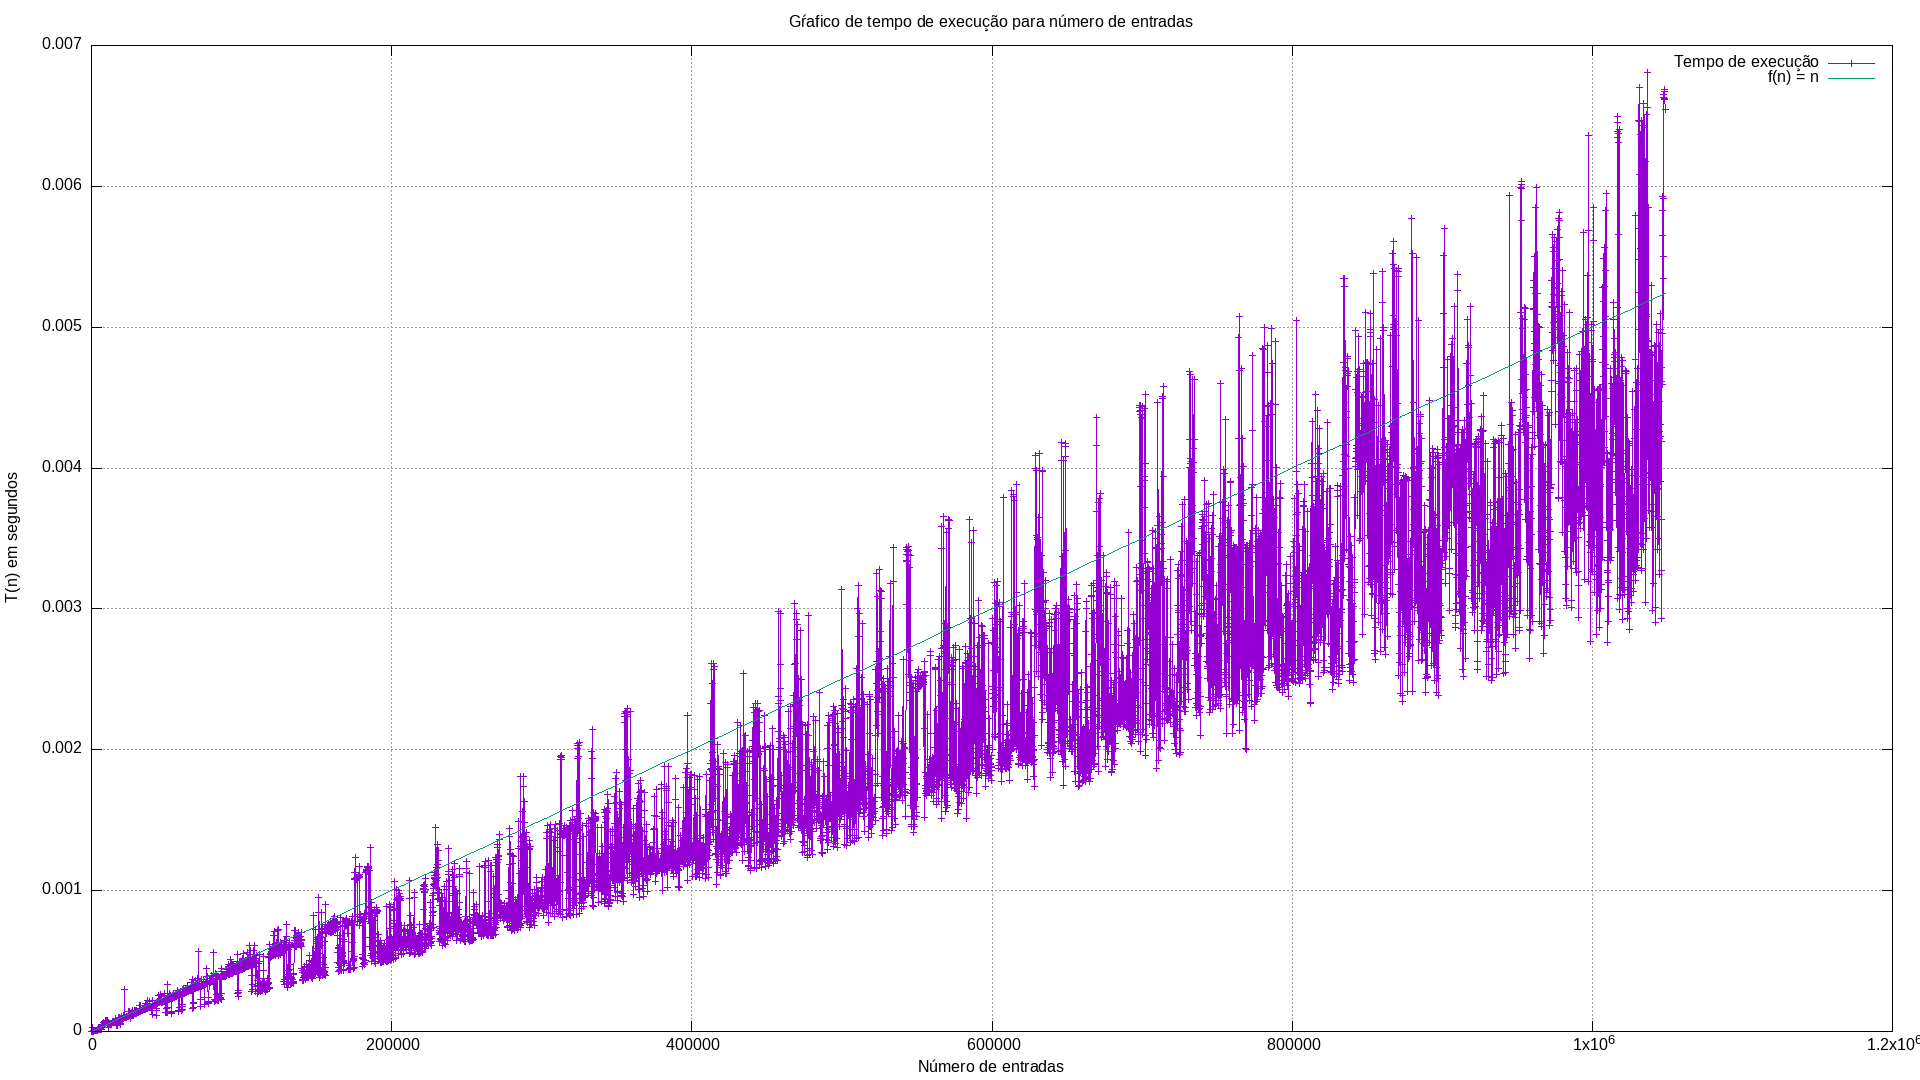
\includegraphics[width=\textwidth]{image/graphics/countingSort.png}
    \caption{Gráfico com tempo de execução do algoritmo de ordenação por contagem}
    \label{cap:2:graph:countingSort}
\end{figure}

No gráfico \ref{cap:2:graph:countingSort}, é possível perceber que o tempo de execução do algoritmo se aproxima
da função $f(n)$ que é uma função linear para $n$ com uma redução de escala para melhor percepção e comparação. Então,
utilizando como base o gráfico \ref{cap:2:graph:countingSort}, pode-se confirmar que a ordem de crescimento determinada é
precisa.

\subsection{Discussão sobre tempo de execução e uso de memória}

Sobre seu tempo de execução, o algoritmo de ordenação por contagem é eficiente para
vetores com muitas entradas desde que exista memória suficiente. Sobre seu uso de memória, é $S(n) = K$.
Como apontado previamente, se por definição, a distância entre o mínimo e o máximo do vetor origem for
relativamente pequena comparada a memória, é um dos melhores algoritmos disponíveis para utilização.



\section{Comparações}

Com as explicações para os algoritmos nas seções (\ref{cap:2:section:isort}, \ref{cap:2:section:ssort}
\ref{cap:2:section:hsort}, \ref{cap:2:section:msort}, \ref{cap:2:section:qsort}, \ref{cap:2:section:csort}),
pode-se racionalizar alguns pensamentos entre os algoritmos. Primeiro, se memória não for um fator relevante,
portanto, ou existe muita memória no computador ou $K$ é uma distância muito pequena, o algoritmo apresentado na
seção \ref{cap:2:section:csort} é o melhor dos apresentados por executar em tempo linear. Se memória for um fator,
dentre os algoritmos da ordem $\Theta(n) = n \log n$, provavelmente quem se sobressai é o algoritmo baseado em
particionamento apresentado na seção \ref{cap:2:section:qsort} porque não utiliza memória auxiliar linear como o \ref{cap:2:section:msort} e
apresenta um comportamento mais estável que o \ref{cap:2:section:hsort} como pode-se observar no gráfico \ref{cap:2:graph:combined}. 
Já, se o número de entradas for quase irrelevante, pode-se aplicar um dos algoritmos de ordem $\Theta(n) = n^2$ 
como os apresentados nas seções (\ref{cap:2:section:isort}, \ref{cap:2:section:ssort}).

\begin{figure}[h]
    \centering
    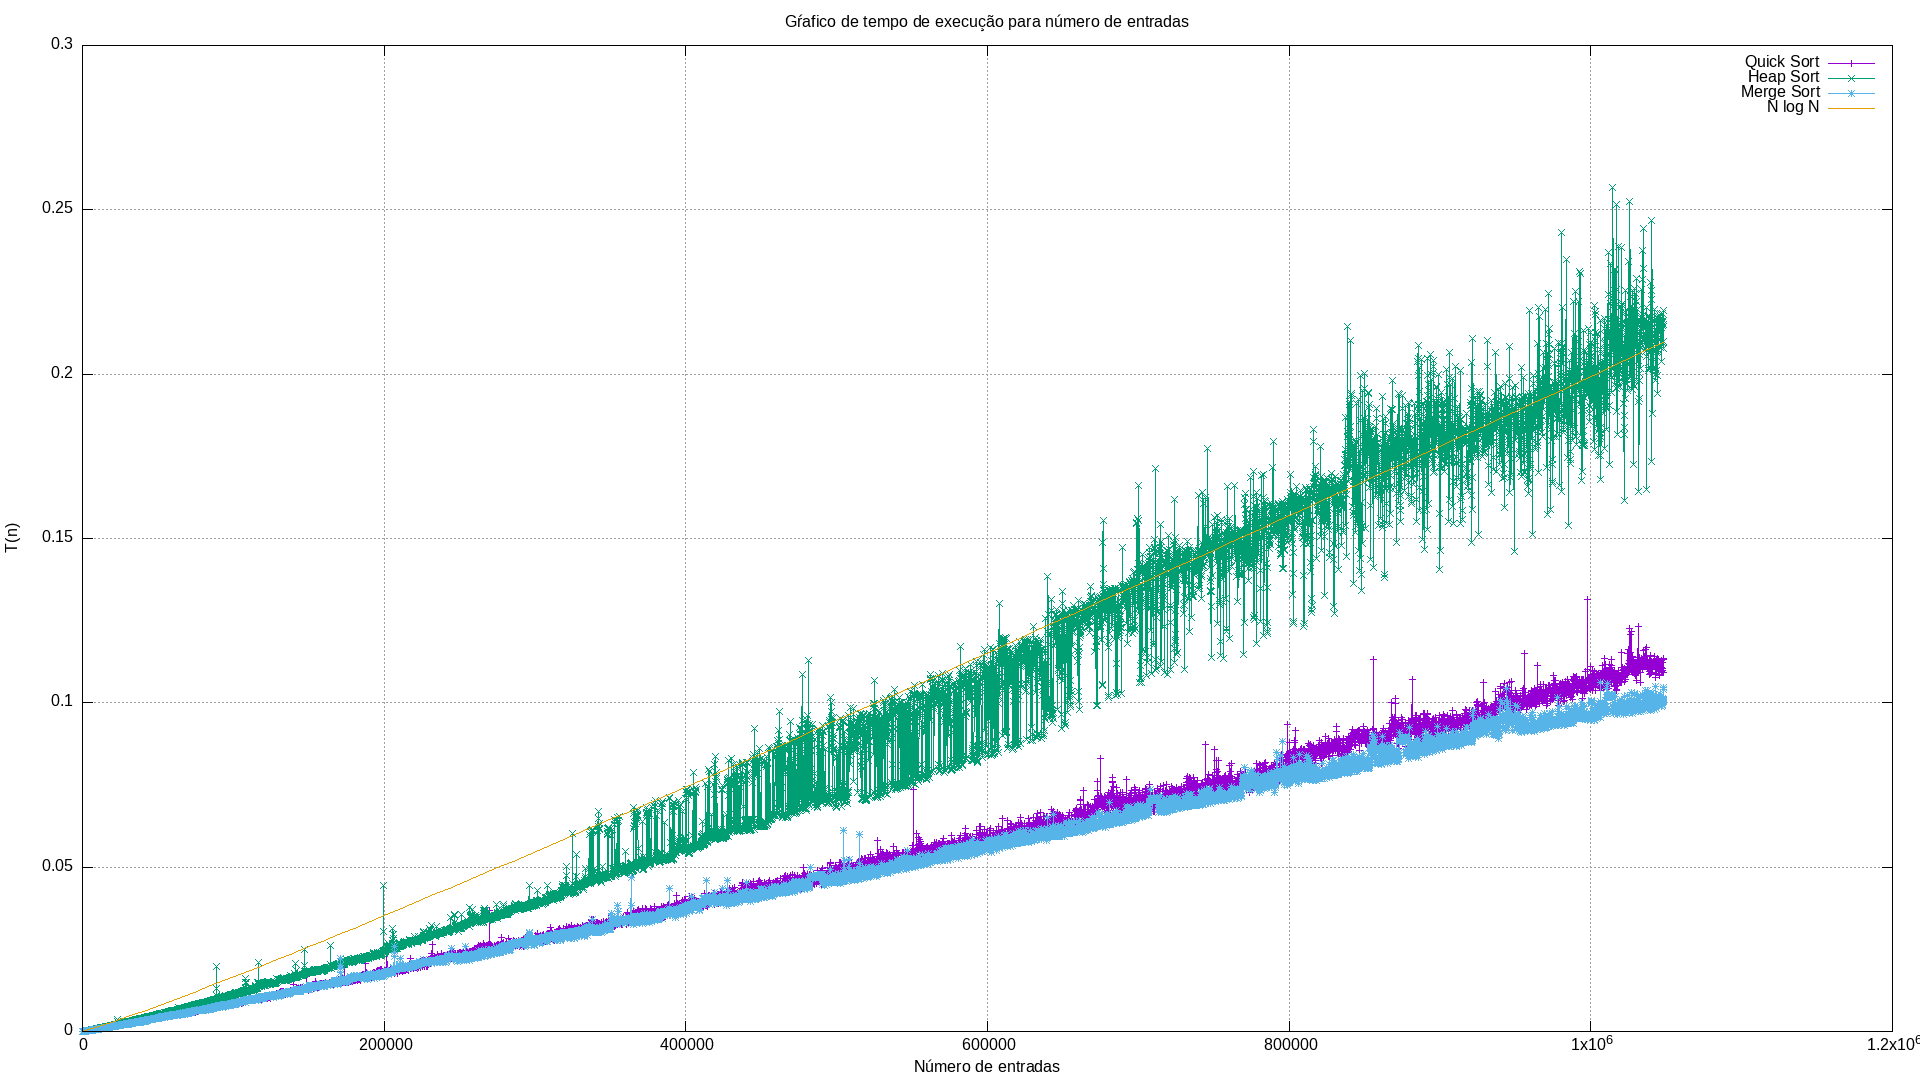
\includegraphics[width=\textwidth]{image/graphics/Combined.png}
    \caption{Gráfico com tempo de execução dos algoritmos n log n}
    \label{cap:2:graph:combined}
\end{figure}

Na tabela \ref{cap:2:table:all}, podemos ver de forma explícita, os tempos de execução e
uso de memória para cada algoritmo.

\begin{table}[h]
    \centering
    \caption{Comparação de algoritmos}
    \label{cap:2:table:all}
    \begin{tabular}{|c|c|c|}
    \hline
    \textbf{Algoritmo} & \textbf{T(n)} & \textbf{S(n)} \\ \hline
    Counting   & $\Theta(n)$    & $\Theta(k)$    \\ \hline
    Quick      & $\Theta(n \log n)$ & $\Theta(1)$   \\ \hline
    Merge      & $\Theta(n \log n)$ & $\Theta(n)$    \\ \hline
    Heap       & $\Theta(n \log n)$ & $\Theta(1)$    \\ \hline
    Insertion  & $\Theta(n^2)$      & $\Theta(1)$    \\ \hline
    Selection  & $\Theta(n^2)$      & $\Theta(1)$    \\ \hline
    \end{tabular}
\end{table}
    


%%%%%%%%%%%%%%%%%%%%%%%%%%%%%%%%%%%%%%%%%%%%%%%%%%%%%%%%%%%%%%%%%%%%%%%%%%%%%
%% FIM CAPÍTULO                                                            %%
%%%%%%%%%%%%%%%%%%%%%%%%%%%%%%%%%%%%%%%%%%%%%%%%%%%%%%%%%%%%%%%%%%%%%%%%%%%%%
